
This section is devoted to fully describe our novel proposal called \textit{Variable Space Diversity based MOEA} 
(\VSDMOEA{})~\footnote{The source code in C++ is freely available in \url{https://github.com/joelchaconcastillo/VSD-MOEA.git}}.
%
The novelty of \VSDMOEA{} appears in the replacement phase, which incorporates
the use of variable space diversity and a novel objective space density estimator. 
%
The main principle behind the design of the novel replacement is to use the stopping criterion and 
elapsed generations with the aim of gradually moving from exploration to exploitation during the search process.
%
Note that this principle might be incorporated in any of the three categories of \MOEAS{}.
%
In this paper, our decision was to incorporate it in a dominance-based approach.
%
Note that this category has been particularly suitable for problems with two and three objectives.
%
Thus, some of our design decisions might not be convenient for dealing with many-objective optimization problems.

The general framework of \VSDMOEA{} is quite standard.
%
Algorithm~\ref{alg:vsd-moea} shows the pseudo-code of \VSDMOEA{}.
%
The parent selection is performed with binary tournament based on the dominance raking with ties broken randomly.
%
The variation stage is based on applying the well-known Simulated Binary Crossover (SBX) 
and polynomial mutation~\cite{Joel:SBX1994, Joel:Mutation}.
%
Thus, the contribution appears in the replacement phase.
%
The rest of this section is devoted to describe the replacement phase, including the novel objective space density 
estimator.

\begin{algorithm}[t]
\algsetup{linenosize=\tiny}
	\caption{Main procedure of VSD-MOEA} 
	\begin{small}
\begin{algorithmic}[1]
 	\STATE \textbf{Initialization}: Generate an initial population $P_0$ with $N$ individuals.
	\STATE \textbf{Evaluation}: Evaluate all individuals in the population.
	\STATE Assign $t=0$
	\WHILE{ (not stopping criterion)  }
	   \STATE \textbf{Mating selection}: Fill the mating pool by performing binary tournament selection on $P_t$, 
		 based on the non-dominated ranks (ties are broken randomly).
	   \STATE \textbf{Variation}: Apply SBX crossover and Polynomial mutation to the mating pool to create a child population $Q_t$.
		 \STATE \textbf{Evaluation}: Evaluate all individuals in $Q_t$.
	   \STATE \textbf{Survivor selection}: Generate $P_{t+1}$ by applying the replacement scheme 
		 described in Algorithm \ref{alg:Replacement_Phase}, using $P_t$ and $Q_t$ as input.
	   \STATE $t=t+1$
	\ENDWHILE
	\end{algorithmic}
	\end{small}
\label{alg:vsd-moea}
\end{algorithm}


\subsection{Replacement Phase of VSD-MOEA}

The replacement phase of \EAS{} is in charge of deciding in each generation which are the survivors 
among the members of the previous population and offspring.
%
The novel replacement promotes a gradual movement from exploration to exploitation, which has been a quite 
beneficial principle in the design of single-objective optimizers~\cite{Joel:MULTI_DYNAMIC}.
%
Particularly, the replacement phase operates as follows.
%
First, the members of the previous population and offspring are joined in a multi-set with $2 \times N$ individuals.
%
Then, an iterative process that selects an additional
individual at each iteration is used to pick up the $N$ survivors. 
%
In order to take into account the diversity of the variable space, the Distance to Closest Survivor (\DCS{}) of each
individual is calculated at each iteration.
%
Thus, the \DCS{} of an individual $I$ is calculated as $\displaystyle{\min_{s \in S}\ Distance(I, s)}$,
where $S$ is the multi-set containing the currently selected survivors. 
%
Normalized Euclidean distances are considered, so in order to calculate distances between any two individuals $A$ and $B$, 
Eq. (\ref{eqn:distance}) is applied.
%
In the first iteration, the $S$ multi-set is empty, so the \DCS{} of each individual is infinity.
%
\begin{equation}\label{eqn:distance}
Distance(A, B) =   \left ( \frac{1}{n}  \sum_{i=1}^n \left ( \frac{A_i - B_i}{x_i^{(U)} - x_i^{(L)}} \right )^2  \right)^{1/2}
\end{equation}

Note that individuals with larger \DCS{} values are those that contribute more significantly to promote exploration.
%
In order to avoid an excessive decrease of the exploration degree, individuals with a \DCS{} value lower 
than a threshold value are penalized.
%
Then, among the non-penalized individuals, an objective space density estimator is used to select the additional
survivor of the iteration.
%
In our case, the novel density estimator described in the next subsection is used. 
%
Note that it might happen that all individuals are penalized.
%
In such a case, the individual with the largest \DCS{} is selected to survive.

\begin{figure}[t]
\centering
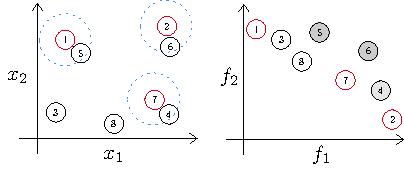
\includegraphics[width=0.45\textwidth]{Images/Diagram.pdf}
\caption{Penalty Method of the Replacement Phase - The left side represents the variables space and the right side the 
objective space.} \label{fig:Hypersphere}
\end{figure}



In order to better understand the penalty method, it can be visualized in the following way.
%
After selecting each survivor, a hyper-sphere 
centered in such a candidate solution --- in the variable space --- is created.
%
Then, all the individuals that are inside a hyper-sphere are penalized and the objective space estimator takes 
into account only the survivors and non-penalized individuals.
%
This is illustrated in Fig.~\ref{fig:Hypersphere}, which represents a state where three individuals have been 
selected to survive and an additional survivor must be picked up.
%
The left side shows individuals in the variable space.
%
Current survivors are marked with a red border and each one of them is surrounded by a blue dash circle with 
radius $D_t$.
%
In this situation, the penalized individuals are the number 4, 5, and 6.
%
In the objective space --- right side --- penalized individuals are shown with gray background, indicating
that the objective space density estimator does not take them into account.

Since using a large radius for the hyper-spheres induces a large degree of 
exploration, it makes sense to reduce this value during the optimization process.
%
This is precisely one of the keys of our proposal.
%
The sizes of the hyper-spheres are modified dynamically by taking into account the stopping 
criterion and elapsed generations.
%
Particularly, the radius is decreased in a linear way starting from an initial distance.
%
This means that in the initial phases exploration is promoted.
%
However, as the size of the radius decreases only very close individuals are penalized, meaning that more 
exploitation is allowed.
%
Note that this method requires a parameter which is the initial radius of the 
hyper-spheres or initial threshold value.
%
This parameter is denoted as $D_I$. 
%
Setting this parameter with a large value might provoke the penalization of a lot of individuals,
thus non-useful diversity might be maintained.
%
However, too small values might not prevent fast convergence and therefore the approach  
might behave as a traditional non-diversity based \MOEA{}.
%
The robustness of the proposal with respect to this additional parameter is studied in our experimental validation.

Algorithm~\ref{alg:Replacement_Phase} formalizes the replacement phase of \VSDMOEA{}.
%
First, the population of the previous generation ($P_t$) and the offspring ($Q_t$) are joined
in $R_t$ (line \ref{alg:1}).
%
The multi-set $R_t$ contains, at each iteration, the remaining non-penalized individuals that might be selected 
to survive.
%
The population of survivors ($P_{t+1}$) and the set containing the penalized individuals are initialized to
the empty set (lines \ref{alg:2} and \ref{alg:3}).
%
Then, the threshold value ($D_t$) that is used to penalize too close individuals is calculated (line \ref{alg:4}).
%
Note that $D_I$ denotes the initial threshold value, $G_{Elapsed}$ is the amount of generations that have 
been evolved, and $G_{End}$ is the stopping criterion, i.e. the number of generations that are to be evolved 
in the execution of \VSDMOEA{}.
%
The linear decrease is calculated so that after the $50\%$ of the generations, the $D_t$ value is lower than 0, 
meaning that no penalties are performed.
%
This means that in the first $50\%$ of the generations, more exploration than in traditional MOEAs is induced.
%

\begin{algorithm}[t]
\algsetup{linenosize=\tiny}
	\caption{Replacement Phase of VSD-MOEA} 
\begin{small}
\begin{algorithmic}[1]
\STATE Input: $P_t$ (Population of current generation), $Q_t$ (Offspring of current Generation)
    	\STATE Output: $P_{t+1}$ 
        \STATE $R_t = P_t \cup Q_t$ \label{alg:1}
        \STATE $P_{t+1} = \emptyset$ \label{alg:2}
        \STATE $Penalized = \emptyset$ \label{alg:3}
				\STATE $D_t = D_I - D_I * \frac{G_{Elapsed}}{0.5*G_{End}}$ \label{alg:4}
        \WHILE{ $|P_{t+1}|$ $\leq$ N } \label{alg:6}
					\STATE Compute $DCS$ of individuals in $R_t$ with $P_{t+1}$ used as reference set \label{alg:7}
					\STATE Move to $Penalized$ the individuals in $R_t$ with $DCS < D_t$  \label{alg:8}
        	\IF{$R_t$ is empty} \label{alg:9}
						\STATE Compute $DCS$ of individuals in $Penalized$ with $P_{t+1}$ used as reference set \label{alg:10}
						\STATE Move to $R_t$ the individual in $Penalized$ with largest $DCS$ \label{alg:11}
        	\ENDIF
					\STATE Identify the first front ($F$) in $R_t \cup P_{t+1}$ with an individual $I \in R_t$ \label{alg:12}
					\STATE Use the novel density estimator (Algorithm~\ref{alg:Density_Estimator}) to select a new survivor 
					from $F$ and move it to $P_{t+1}$\label{alg:13}
        \ENDWHILE
    	\RETURN $P_{t+1}$ \label{alg:14}
	\end{algorithmic}
\end{small}
\label{alg:Replacement_Phase}
\end{algorithm}

Then, an iterative process that selects an individual at each iteration is executed until the survivors
set contains $N$ individuals (line \ref{alg:6}).
%
The iterative process works as follows.
%
First, the \DCS{} value of each remaining non-penalized individual is calculated (line \ref{alg:7}).
%
Then, those individuals with a \DCS{} value lower than $D_t$ are moved to the set of penalized individuals (line \ref{alg:8}).
%
If all the remaining individuals are penalized (line \ref{alg:9}), it means that the amount of exploration is lower than the
desired one.
%
Thus, the individual with the largest \DCS{} value is recovered, i.e. moved to the non-penalized individuals 
set (lines \ref{alg:10} and \ref{alg:11}) and consequently it survives.
%
Finally, the objective space is taken into account.
%
Specifically, candidate non-penalized individuals and current survivors are joined.
%
Then, the well-known non-dominated sorting procedure~\cite{Joel:NSGAII} is executed with such a set, stopping as soon as a front with 
a candidate individual is found, i.e. with an individual of $R_t$ (line \ref{alg:12}).
%
Then, taking the identified front as input, a novel objective space density estimator is used to select
the next survivor (line \ref{alg:13}).
%
The specific way in which the contribution to diversity of the objective space of each individual is measured is described in the next section.
%

\subsection{A Novel Density Estimator for the Objective Space}
\label{subsection:density}

\begin{algorithm}[t]
\algsetup{linenosize=\tiny}
	\caption{Density estimator} 
\begin{small}
\begin{algorithmic}[1]
\STATE Input: $P_{t+1}$ (Survivors), $R_t$ (Candidates), $F$ (Current front)
    	\STATE Output: $I \in R_t$ 
	\STATE $FP = P_{t+1} \cap F$ \label{alg:FP}
	\STATE $FR = R_{t} \cap F$ \label{alg:FR}
        \FOR{$k \in$ number of objectives}\label{alg:density_for}
	      \STATE Select the best individual $I \in F$ of $k$ according to Eq.~\ref{eqn:extremes}.\label{alg:density_1}
	  	\IF{ $I \in FR$}
	  	 \RETURN $I$ \label{alg:density_2}
	  	\ENDIF
	\ENDFOR\label{alg:density_endfor}
	\STATE $MaxID = 0$ \label{alg:density_for2}
	\FOR{ $ Ic \in FR$}
	\STATE $Improvement = \displaystyle{\min_{s \in FP}\ ID(Ic, s)}$ 
	\IF{ $Improvement > MaxID$} \label{alg:density_if2}
	   \STATE $MaxID = Improvement$
	   \STATE $I = Ic$ 
	\ENDIF \label{alg:density_endif2}
	\ENDFOR	\label{alg:density_endfor2}
    	\RETURN $I$ \label{alg:density_4}
	\end{algorithmic}
\end{small}
\label{alg:Density_Estimator}
\end{algorithm}

Since the dominance definition is not related to the preservation of diversity of the objective space,
dominance-based \MOEAS{} usually incorporate objective-space density estimators to promote the survival
of diverse individuals.
%
As it was previously described, our density estimator selects a new survivor from the front identified
in line \ref{alg:13} of Algorithm~\ref{alg:Replacement_Phase}.
%
This front (referred in Algorithm~\ref{alg:Density_Estimator}  as $F$) contains at least one individual belonging to $R_t$ and it might also contain some elements 
of $P_{t+1}$.
%
The aim behind the selection of the next survivor is to pick up an individual of the input front
that contributes significantly in terms of objective-space quality and diversity. % to $R_t$.

Algorithm~\ref{alg:Density_Estimator} describes the selection of the next survivor.
%
First, the sets $FP$ and $FR$ are identified (lines \ref{alg:FP} and \ref{alg:FR}).
%
$FP$ contains the current survivors that are in $F$, whereas $FR$ contains
the remaining non-penalized individuals that are in $F$.
%
Then, similarly to most state-of-the-art algorithms, an action to promote the selection of boundary solutions
is included.
%
Note that selecting the best solution for each objective might provoke some drawbacks related to accepting a small improvement
in an objective at the cost of important worsenings in other objectives~\cite{deb2016optimality}.
%
To solve this issue augmented functions can be applied, which has been the alternative used in this paper.
%
Particularly, iteratively, for each objective $k$ the candidate solution that minimizes the Augmented Function (AF)
given in Eq.~\ref{eqn:extremes} is identified (lines \ref{alg:density_for} to \ref{alg:density_endfor}).
%
If such an individual belongs to $FR$, i.e., it has not been selected yet as a survivor, the next survivor is such an individual
and the process finalizes (line \ref{alg:density_2}).
%
Note that, augmented functions usually take into account weight vectors with the aim of dealing with objectives
that present very different scales.
%
Since benchmarks that have similar scales in each objective have been used in this paper, there was no need to apply
such weight vectors.

\begin{equation}\label{eqn:extremes}
AF_k (\vec{x}) = f_k(\vec{x}) + 10^{-4} \times  \sum_{j=1}^M f_j( \vec{x} )
\end{equation}

In cases where the individuals that optimize each $AF_K$ function are already in $P_{t+1}$, a contribution
to objective-space diversity is calculated for each individual in $FR$ (lines \ref{alg:density_for2} to \ref{alg:density_4}).
%
This contribution is calculated by taking into account the current survivors of the front ($FP$).
%
Particularly, the ``Improvement Distance'' ($ID$) defined for the indicator IGD+~\cite{Joel:Inverted_Generational_Distance_Plus}
is used.
%
The $ID$ of an individual $A$ with respect to an individual $B$ is calculated by taking into account only the objectives
where $A$ is better.
%
Specifically, Eq. (\ref{eq:ImprovementDistance}) is used.

\begin{equation} \label{eq:ImprovementDistance}
\begin{split}
 ID(A, B) = &  \left (\sum_{i=1}^M \left (max(0, B_i - A_i \right ))^2  \right)^{1/2}
\end{split}
\end{equation}

The contribution of each member of $FR (I)$ is calculated as $\displaystyle{\min_{s \in FP}\ ID(I, s)}$.
%
Then, the individual with the highest contribution is selected as the next survivor (lines \ref{alg:density_if2} to \ref{alg:density_endif2}).%, with ties broken randomly (line XXX).

